\section{Vektoren}

Ein Vektor beschreibt eine Strecke mit Richtung zwischen 2 Punkten im Raum.
Ein Vektor kann von jedem Ort im Raum ausgehen.und hat immer einen Start- und Endpunkt. 
Jeder Punkt im Raum lässt sich als Vektor vom Ursprung $O$ zu den Koordinaten des Punktes
darstellen.

\begin{equation*}
    P (1, 3, 2) \rightarrow \overrightarrow{OP} = \begin{bmatrix}
        1 \\
        3 \\
        2
    \end{bmatrix}
    \qquad A (1, 2, 2) \; B (4, 3, 1) \rightarrow \overrightarrow{AB} = \begin{bmatrix}
        3 \\
        1 \\
        -1
    \end{bmatrix}
\end{equation*}

\subsection{Rechnen mit Vektoren}

\subsubsection{Addition und Subtraktion}

\subsubsection{Länge eines Vektor}

Die Länge eines Vektors ergibt sich aus dem Satz des Pythagoras.
Betragsstriche um einen Vektor bedeuten, dass dessen Länge gemeint ist.

\begin{equation*}
    \overrightarrow{AB} = \begin{bmatrix}
        3 \\
        1 \\
        -1
    \end{bmatrix}
    \qquad | \overrightarrow{AB} | = \sqrt{3^2 + 1^2 + (-1)^2} = \sqrt{11}
\end{equation*}

\subsection{Kollineare Vektoren}

\subsection{Differenzvektor}

\subsection{Abstand von Punkten}

\subsection{Mittelpunkt einer Strecke}

\subsection{Skalarprodukt}

Das Skalarprodukt ist die Summe der Produkte der einzelnen Vektorelemente.
Das Ergebnis ist eine relle Zahl.

\begin{equation*}
    \begin{bmatrix}
        3 \\
        1 \\
        -1
    \end{bmatrix} \cdot
    \begin{bmatrix}
        2 \\
        0 \\
        -1
    \end{bmatrix} = 3 \cdot 2 + 1 \cdot 0 + -1 \cdot -1 = 7
\end{equation*}

\subsubsection{Winkel beim Skalarprodukt}

\subsubsection{Kollineare Vektoren beim Skalarprodukt}

\subsubsection{Skalarprodukt Assoziativ, Kommutativ, Distributiv}

\clearpage

\subsection{Kreuzprodukt}

Das Kreuzprodukt zweier Vektoren ergibt einen dritten Vektor der orthogonal
zu beiden anderen ist. Das Kreuzprodukt von Rot-Blau ist der Vektor Pink, orthogonal zur
Ebene von Rot-Blau.

\begin{equation*}
    \vec{a} \times \vec{b} =
    \begin{bmatrix}
        a_1 \\
        a_2 \\
        a_3
    \end{bmatrix} \times
    \begin{bmatrix}
        b_1 \\
        b_2 \\
        b_3
    \end{bmatrix} =
    \begin{bmatrix}
        a_2 b_3 - a_3 b_2 \\
        a_3 b_1 - a_1 b_3 \\
        a_1 b_2 - a_2 b_1
    \end{bmatrix}
\end{equation*}

\begin{equation*}
    \begin{bmatrix}
        3 \\
        1 \\
        -1
    \end{bmatrix} \times
    \begin{bmatrix}
        2 \\
        0 \\
        -1
    \end{bmatrix} =
    \begin{bmatrix}
        1 \cdot (-1) - (-1) \cdot 0 \\
        (-1) \cdot 2 - 3 \cdot (-1) \\
        3 \cdot 0 - 1 \cdot 2
    \end{bmatrix} =
    \begin{bmatrix}
        -1 \\
        1 \\
        -2
    \end{bmatrix}
\end{equation*}

\begin{center}
    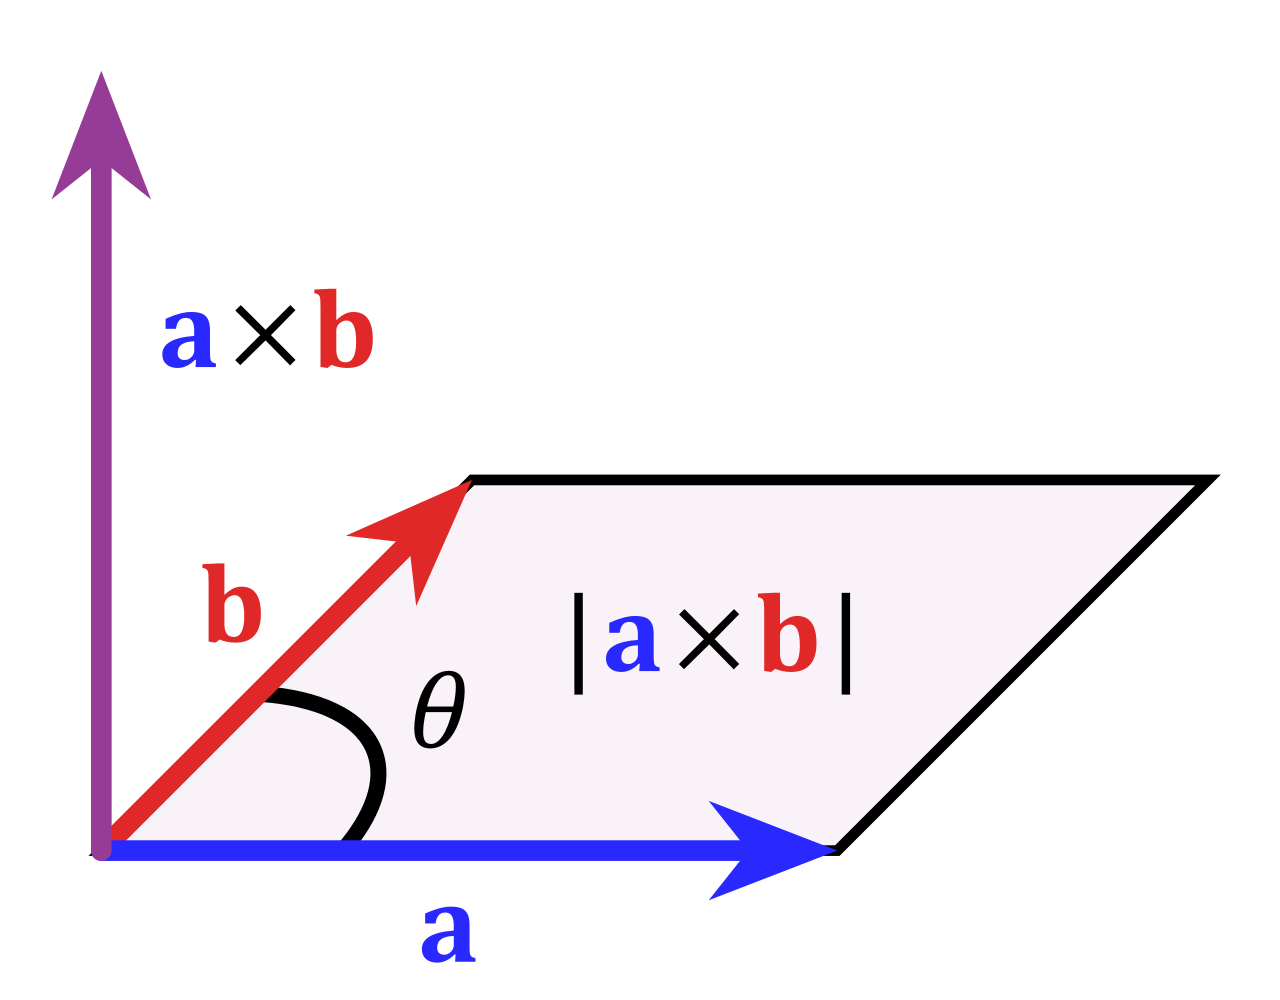
\includegraphics[width=0.6\textwidth]{images/cross-p.png}
\end{center}


\section{3D Koordinatensystem}
\subsection{2 Varianten}
\subsection{Punkte Ablesen}
\subsection{Punkte Einzeichnen}

\section{Spiegelungen}
\subsection{2D Spiegelungen}
\subsubsection*{Achsenspiegelung}
\subsubsection*{Punktspiegelung}
\subsection{3D Spiegelungen}
\subsubsection*{Ebenenspiegelung}
\subsubsection*{Punkspiegelung}
\subsubsection*{Achsenspiegelung}

\section{Geraden}
\subsection{Geradengleichung}
\subsection{Geradengleichung aus 2 Punkten Aufstellen}
\subsubsection{Mehrdeutigkeit von Geradengleichung}
\subsubsection{2D / 3D}
\subsection{Spurpunkte auf Koordinatenebenen}
\subsection{Lagebeziehungen von Geraden}
\subsubsection{Parallelität von Geraden}
\subsubsection{Identische Geraden}
\subsubsection{Schnittpunkt von Geraden}
\subsubsection{Windschiefe Geraden}

\section{Ebenen}
\subsection{Formen von Ebenen}
\subsection{Parameterform, Normalenform, Koordinatenform bei Ebenengleichungen}
\subsection{Umwandlung zwischen den Formen}
\subsection{Lagebeziehung Punkt-Ebene}
\subsection{Punktprobe für Ebene}
\subsection{Lagebeziehung Gerade und Ebene}
\subsection{Schnittpunkt, Parallel, Gerade liegt in Ebene}
\subsection{Lagebeziehung Ebene und Ebene}
\subsection{Schnittgerade, Parallel, Ebene liegt in Ebene}
\subsection{Winkel bei Geraden, Vektoren und Ebenen}
\subsection{Winkel Gerade - Gerade}
\subsection{Winkel Ebene - Ebene}
\subsection{Winkel Gerade - Ebene}
\subsection{Kürzester Abstand Punkt, Gerade (Analysis, Skalarprodukt)}
\subsection{Kürzester Abstand Punkt, Ebene}
\subsection{Parallele Geraden, Parallele Ebenen, Gerade parallel zu Ebene}
\subsection{Abstand Windschiefer Geraden}







